
\chapter{PENDAHULUAN}
\label{cha:1-Pendahuluan}

\section{Latar Belakang}
\label{sec:1-LatarBelakang}

Bagian ini menceritakan latar belakang dari penelitian.
Bagian ini menceritakan latar belakang dari penelitian.
Bagian ini menceritakan latar belakang dari penelitian.
Bagian ini menceritakan latar belakang dari penelitian.
Bagian ini menceritakan latar belakang dari penelitian.
Bagian ini menceritakan latar belakang dari penelitian.
Bagian ini menceritakan latar belakang dari penelitian.
Bagian ini menceritakan latar belakang dari penelitian.
Bagian ini menceritakan latar belakang dari penelitian.
Bagian ini menceritakan latar belakang dari penelitian.
Bagian ini menceritakan latar belakang dari penelitian.
Bagian ini menceritakan latar belakang dari penelitian.
Bagian ini menceritakan latar belakang dari penelitian.
Bagian ini menceritakan latar belakang dari penelitian.
Bagian ini menceritakan latar belakang dari penelitian.


\section{Batasan dan Tujuan}
\label{sec:1-BatasTujuan}

Bagian ini menceritakan tentang :
\begin{itemize}
\item Batasan penelitian beserta alasannya.
\item Definisi permasalahan dari penelitian
\item Tujuan umum dan khusus dari penelitian
\end{itemize}

 
\begin{figure}[tb]
\vspace{-0.3cm}
%\rule{\columnwidth}{0.1pt}
\begin{center}
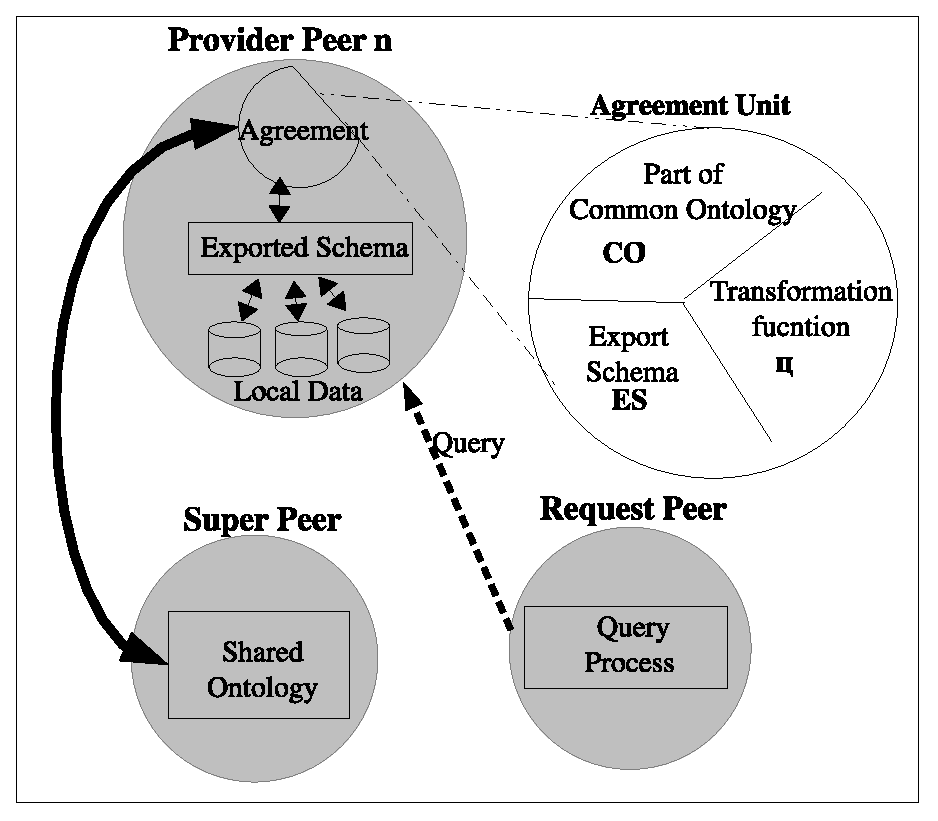
\includegraphics[width=0.7\columnwidth]{bab1/ContohGbr1_1.eps}
\end{center}
\vspace{-0.5cm}
%\rule{\columnwidth}{0.1pt}
\caption{\small Contoh 1.1 untuk menampilkan gambar \label{fig:1-contoh1.1}}
\end{figure}


\section{Kontribusi}
\label{sec:1-Kontribusi}
Menjelaskan kontribusi utama dari hasil penelitian.

\textit{\textbf{Ini mendemonstrasikan fungsi label untuk mengacu kepada sebuah gambar. Lihat gambar \ref{fig:1-contoh1.1} sebagai contoh awal. Contoh referensi lihat referensi \cite{Sheth:b}}
}